%==============================================================================
% Paper 1 — Medical Image Analysis (Elsevier)
%
% Target: Medical Image Analysis, single-column, ~10–15 pages, Harvard
%         author-year citations.
% Status: data-complete. Only remaining author task is the funding line
%         in the Acknowledgements.
%==============================================================================

\documentclass[review,1p,times]{elsarticle}

% ---------- Packages ----------------------------------------------------------
\usepackage{amsmath,amssymb,amsfonts}
\usepackage{graphicx}
\usepackage{booktabs}
\usepackage{multirow}
\usepackage{makecell}
\usepackage{array}
% siunitx removed -- tables now use plain c columns
\usepackage{xcolor}
\usepackage{hyperref}
\hypersetup{colorlinks=true,linkcolor=blue,citecolor=blue,urlcolor=blue}
\usepackage{enumitem}
\usepackage{subcaption}
% Note: elsarticle already loads natbib; do not load it again.

% Draft-review annotation commands (only \TODO remains in use, for the
% single outstanding funding line in the Acknowledgements)
\newcommand{\TODO}[1]{\textcolor{red}{\textbf{[TODO: #1]}}}
\newcommand{\PLACE}[1]{\textcolor{orange}{\textbf{[PLACEHOLDER: #1]}}}
\newcommand{\REVIEW}[1]{\textcolor{blue}{\textbf{[REVIEW: #1]}}}

% Math operators
\DeclareMathOperator{\Dice}{Dice}
\DeclareMathOperator{\HD}{HD}
\DeclareMathOperator{\ASSD}{ASSD}

% Bibliography style: MedIA uses Harvard (author-year)
\bibliographystyle{elsarticle-harv}

\journal{Computers in Biology and Medicine}

%==============================================================================
\begin{document}

\begin{frontmatter}

\title{A Comprehensive Benchmark of Deep Learning Architectures for
       2D Echocardiographic Segmentation:\\
       From CNNs to Transformers}

% ---------- Authors -----------------------------------------------------------
\author[a]{Fares Sofiane Mazouni\corref{cor1}}
\ead{faressofiane.mazouni@univ-tebessa.dz}
\cortext[cor1]{Corresponding author.}

\author[a]{Mohamed Yacine Haouam}
\ead{mohamed-yassine.haouam@univ-tebessa.dz}

\author[a]{Mohamed Amroune}
\ead{mohamed.amroune@univ-tebessa.dz}

\author[a]{Issam Bendib}
\ead{issam.bendib@univ-tebessa.dz}


\address[a]{Laboratory of Mathematics, Informatics and Systems (LAMIS), Echahid Cheikh Larbi Tebessi University, Tebessa, 12002, Algeria}

% ---------- Abstract ----------------------------------------------------------
\begin{abstract}
%
Two-dimensional echocardiography is the most widely used cardiac imaging
modality, but quantitative analysis is hampered by speckle noise, low
boundary contrast, and inter-observer variability. U-Net descendants,
attention-augmented CNNs, hybrid CNN--Transformer designs, and pure
Transformer networks all report strong results on this task, yet direct
comparison between them is confounded by inconsistent training protocols
and evaluation pipelines.
%
We benchmark nine representative architectures spanning three paradigms
under one training protocol, one data split, and one evaluation pipeline
on the CAMUS dataset, reporting per-class Dice and IoU, boundary distances
in millimetres, biplane Simpson's ejection fraction (EF) error,
phase-stratified and image-quality-stratified results, efficiency, and
Bonferroni-corrected Wilcoxon tests.
%
Two findings stand out. First, boundary accuracy has saturated: the best
architecture reaches HD95 $= 4.08$~mm against a published CAMUS baseline
of $\approx 4.3$~mm, and the three best architectures lie within $0.2$~mm of
one another, well inside training variance. Clinical agreement is bounded by the
measurement rather than by the network: applying the official CAMUS biplane
pipeline to the ground-truth masks gives EF MAE $= 5.44\%$, and the best
architecture reaches $6.62\%$. Segmentation therefore contributes about
$1.2$ points of EF error on top of a $5.4$-point floor that no model can
cross, and the spread across all nine architectures is $4.0$ points. Neither
axis leaves much headroom for architectural change.
%
Second, we identify a reporting error that makes cross-paper boundary
comparison unreliable. Computing Hausdorff distances on the network's
resized grid while applying the native image spacing under-reports every
distance by the resampling factor --- on CAMUS, $\approx 2.2\times$. Under
that convention our own models score below $2$~mm, which would appear to
halve the published baseline; scored at native resolution the same
predictions merely match it. Any sub-$2$~mm HD95 reported on CAMUS
warrants checking against this failure mode.
%
Code, checkpoints, and per-patient predictions are publicly released.
%
\end{abstract}

\begin{keyword}
medical image segmentation \sep echocardiography \sep CAMUS \sep
deep learning benchmark \sep U-Net \sep Swin Transformer \sep TransUNet
\end{keyword}

\end{frontmatter}

%==============================================================================
% Body
%==============================================================================

%==============================================================================
\section{Introduction}
\label{sec:introduction}

Two-dimensional echocardiography is the most widely used cardiac imaging
modality worldwide: it is portable, inexpensive, non-ionising, and provides
real-time visualisation of cardiac structure and function. Its core
quantitative output --- left ventricular ejection fraction (LVEF), computed
from end-diastolic and end-systolic volumes via the biplane Simpson's method
\citep{lang2015} --- drives a large fraction of clinical cardiac decisions,
from diagnosis of heart failure to monitoring of cardiotoxic chemotherapy.
The clinical importance of LVEF is matched by the operator-dependent
nature of its measurement: published inter-observer LVEF variability is
approximately $7$--$10\%$ \citep{leclerc2019}, which directly limits the
sensitivity of LVEF as a clinical decision boundary.

Automated segmentation of the left ventricular endocardium (LV-endo),
epicardium (LV-epi), and left atrium (LA) from two-dimensional apical
2-chamber (2CH) and 4-chamber (4CH) views would, in principle, eliminate
this operator-dependent variability and provide reproducible volumetric
measurements. The technical challenge is substantial: ultrasound suffers
from low signal-to-noise ratio, speckle noise, low boundary contrast,
acoustic shadowing, and view-dependent geometric foreshortening.

\paragraph{Architectural pluralism.}
Three paradigms have emerged as competitive solutions in this space:
\begin{itemize}[leftmargin=*,nosep]
\item \textbf{Pure convolutional networks.} U-Net
      \citep{ronneberger2015} and its descendants (residual encoders, SE
      blocks, attention gates, deep supervision)
      \citep{milletari2016,oktay2018} remain the dominant architectural
      family, with nnU-Net \citep{isensee2021} serving as a strong
      auto-configured baseline.
\item \textbf{Hybrid CNN--Transformer networks.} TransUNet
      \citep{chen2021transunet} and similar hybrids combine a
      convolutional encoder with a Vision Transformer bottleneck,
      explicitly trading off local detail (CNN) against global context
      (self-attention).
\item \textbf{Pure Transformer networks.} Swin-UNet \citep{cao2022}
      replaces the convolutional \emph{backbone} with a hierarchy of
      windowed self-attention blocks --- retaining only a shallow
      convolutional patch-embedding stem --- demonstrating that
      predominantly attention-based encoders can match or exceed CNN
      performance on a range of medical tasks.
\end{itemize}

\paragraph{The benchmarking gap.}
Despite this architectural pluralism, the literature offers no
systematic, like-for-like comparison of these three paradigms on a single
shared evaluation pipeline. Each paper introducing a new architecture
typically compares against a small number of baselines under different
training protocols, augmentations, learning-rate schedules, and
evaluation metrics. As a result it is difficult for clinicians or
practitioners to answer a basic question: \emph{which architectural
family should I use for CAMUS-style apical 2D echocardiographic
segmentation, and what are the trade-offs?}

This paper provides that comparison on the CAMUS dataset
\citep{leclerc2019}, the standard public 2D echocardiographic
segmentation benchmark, with 500 patients across two views and two
cardiac phases. We train nine representative architectures spanning the
three paradigms above using one identical protocol --- same optimiser,
loss, schedule, augmentation, mixed-precision settings, and early-stopping
criterion --- and evaluate them on a single shared pipeline reporting
geometric, boundary, clinical, and efficiency metrics simultaneously.

\paragraph{Contributions.}
\begin{itemize}[leftmargin=*,nosep]
\item We present the first unified, like-for-like benchmark of deep
      segmentation architectures on CAMUS across the three major paradigms:
      nine architectures spanning pure CNN, hybrid CNN--Transformer, and
      pure Transformer, trained and evaluated under a single shared protocol.

\item We report \emph{multi-dimensional} evaluation, going beyond Dice
      to include HD95 in millimetres (with per-sample NIfTI pixel
      spacing), ASSD, biplane Simpson's EF MAE and Pearson $r$, ED/ES
      stratified metrics, robustness across CAMUS image-quality grades,
      and efficiency benchmarks (parameters, FLOPs, latency, peak
      memory). The full results matrix and per-patient outputs are
      released.

\item We apply pairwise Wilcoxon signed-rank tests with Bonferroni
      correction to identify which architectural differences are
      statistically significant, and produce a critical-difference
      diagram showing the top-tier band of equivalent models.

\item \textbf{We document a boundary-metric reporting error that makes
      published HD95 values on CAMUS mutually incomparable.} Computing
      the distance transform on the network's resized $256 \times 256$
      grid while attaching the native NIfTI spacing under-reports every
      distance by the resampling factor, which on CAMUS is
      $\approx 2.2\times$. The effect is large enough to invert a
      conclusion: under that convention our models score
      $1.8$--$2.9$~mm and appear to halve the published baseline, while
      the identical predictions scored at native resolution give
      $4.1$--$5.7$~mm and merely match it. We report both, and recommend
      that boundary distances be computed at acquisition resolution ---
      a concrete instance of the validation concerns raised by
      \citet{reinke2021limitations} and \citet{maierhein2024metrics}.

\item Our best architecture, TransUNet, reaches Dice $= 0.9121$,
      HD95 $= 4.08$~mm; nnU-Net reaches Dice $= 0.9099$, HD95 $= 4.27$~mm
      with $6.5\times$ fewer parameters and roughly $3\times$ faster
      inference. Boundary accuracy under our unified protocol reproduces
      the originally published nnU-Net baseline
      ($\approx 4.3$~mm) \citep{leclerc2019} rather than improving on it,
      and EF is floor-limited in the same way: the ground-truth oracle
      scores $5.44\%$ MAE under an identical pipeline against the best
      model's $6.62\%$, leaving roughly $1.2$ points attributable to
      segmentation at all.

\item We release a fully reproducible benchmark framework: training,
      evaluation, statistical analysis, and figure generation code.
\end{itemize}

\paragraph{Outline.}
Section~\ref{sec:related} reviews segmentation architectures and the
CAMUS benchmark. Section~\ref{sec:methods} describes the nine
architectures, the unified training protocol, and the evaluation
pipeline. Section~\ref{sec:results} reports the experimental results.
Section~\ref{sec:discussion} discusses architectural design choices,
trade-offs, and limitations. Section~\ref{sec:conclusion} concludes.

%==============================================================================
\section{Related Work}
\label{sec:related}

\subsection{Convolutional segmentation networks}
\label{sec:related-cnn}

U-Net \citep{ronneberger2015} established the encoder--decoder
architecture with skip connections that remains the dominant template for
medical image segmentation. Subsequent work has refined the encoder
(residual blocks / ResNet \citep{he2016} and later compound-scaled
backbones), the decoder
(transposed convolution vs.\ bilinear upsampling, dense connections
\citep{huang2017}), and the skip mechanism
(attention gates \citep{oktay2018}, dense skips). Squeeze-and-excitation
blocks \citep{hu2018} provide channel-wise recalibration. Atrous spatial
pyramid pooling (ASPP) in DeepLabV3+ \citep{chen2018encoder} replaces the
deep encoder with dilated convolutions to enlarge the receptive field
without down-sampling. Feature Pyramid Networks
\citep{lin2017} aggregate features across multiple scales for dense
prediction.

The nnU-Net framework \citep{isensee2021} integrates these architectural
choices with automatic data-dependent hyperparameter selection (target
spacing, patch size, batch size, augmentation pipeline) and has set
strong baselines on numerous medical benchmarks including CAMUS.

\subsection{Transformer-based segmentation networks}
\label{sec:related-trans}

Self-attention's quadratic complexity made global attention impractical
for high-resolution images until Vision Transformers
\citep{dosovitskiy2021} demonstrated patch-based tokenisation. TransUNet
\citep{chen2021transunet} was the first work to bring this design to
medical segmentation, combining a CNN encoder (typically ResNetV2-BiT
\citep{kolesnikov2020}) with a ViT-B/16 bottleneck and a cascaded
upsampler decoder. The hybrid design retains the inductive bias of
convolutions at high resolution while granting global context at the
bottleneck.

Swin Transformer \citep{liu2021swin} introduced windowed self-attention
with shifted windows, restoring linear complexity in image size. Swin-UNet
\citep{cao2022} adapts this to segmentation with a fully Transformer-based
U-Net. SwinV2 \citep{liu2022swinv2} and Swin-MAE
\citep{baochen2023swinmae} further refine pretraining strategies.

\subsection{Echocardiographic segmentation and CAMUS}
\label{sec:related-camus}

The CAMUS dataset \citep{leclerc2019} (\emph{Cardiac Acquisitions for
Multi-structure Ultrasound Segmentation}) provides 2D apical-2-chamber and
apical-4-chamber acquisitions from 500 patients, each annotated by an
expert echocardiographer at end-diastole and end-systole with four
classes (background, LV-endo, LV-epi, LA). The official split assigns
$400$ patients to training, $50$ to validation, and $50$ to test, with
test annotations held out by the challenge organisers. Image quality is
graded into \emph{Good}, \emph{Medium}, and \emph{Poor} categories by
the same experts.

The original CAMUS paper reported nnU-Net achieving
HD $\approx 4.3$~mm on LV-endo and $\sim$$9\%$ EF MAE.
Subsequent work \citep{painchaud2022, smistad2021}
has reported incremental improvements using deeper architectures, custom
losses, and view-aware training. Several papers have additionally
explored sequence-aware models on CAMUS half-cycle annotations
\citep{painchaud2022}, but these are out of scope for the present
benchmark.

Activity on echocardiographic segmentation has continued along four
largely separate lines. The first pursues \emph{architectural} refinement:
bi-directional token matching between frames \citep{liu2025botm},
dynamic-learning U-Nets that enforce temporal consistency across the
cardiac cycle \citep{qu2025dylunet}, contour-guided query-based fusion
aimed explicitly at boundary quality \citep{ullah2026contour}, and
selective state space models applied to paediatric echocardiography
\citep{ye2024pmamba}. The second addresses \emph{domain shift}, which is
the dominant obstacle to deploying any of these models across scanners
and sites: reinforcement-learning-based domain adaptation
\citep{judge2024domain, judge2025rlda} and interpretable quantification of
the shift itself \citep{elyasi2026domainshift}. The third applies
\emph{foundation models} and self-supervision, either by adapting
general-purpose promptable segmenters to medical images
\citep{ma2024samed}, by generating synthetic cardiac ultrasound for
augmentation \citep{tiago2024synthetic, reynaud2025echoflow}, or by asking
what self-supervised echocardiographic representations actually transfer
\citep{majchrowska2026ssl}. The fourth targets the \emph{clinical
endpoint} directly, predicting or explaining ejection fraction rather than
the mask that produces it \citep{zhang2024lvpredict, thomas2024echonarrator,
li2025echovlm, wang2026echoagent}.

What these lines share is a comparison protocol inherited from whichever
baseline was convenient. Each reports its own training recipe, its own
resolution, and — as we show in Section~\ref{sec:results-boundary} — not
always the same definition of a millimetre. That is the gap this benchmark
addresses.

EchoNet-Dynamic \citep{ouyang2020} provides a complementary large-scale
video dataset for EF regression. We focus on CAMUS as the standard
benchmark for \emph{segmentation-derived} EF. Because EchoNet-Dynamic
annotates only the left-ventricular endocardium in a single apical view,
it cannot exercise the LV-epicardium, left-atrium, or biplane-EF
components of our protocol; whether the architectural trade-offs reported
here transfer to other echocardiographic cohorts is therefore a question
we leave to future cross-dataset work rather than a claim we make here.

\subsection{Validation practice and metric reporting}
\label{sec:related-validation}

Running alongside the architectural literature is a smaller body of work
arguing that the field's \emph{measurement} practice, not its model
design, is now the limiting factor. \citet{reinke2021limitations} catalogue
the ways standard segmentation metrics mislead when applied without regard
to structure size, shape, or resolution, and the Metrics Reloaded
framework \citep{maierhein2024metrics} turns that catalogue into
problem-driven recommendations for choosing and reporting them.
\citet{isensee2024revisited} show that much of the reported progress in 3D
medical segmentation dissolves under rigorous validation, with a
well-configured U-Net still matching or beating architectures claimed to
supersede it. \citet{kazaj2025claims} reach a similar conclusion for the
CNN-versus-Transformer-versus-Mamba question specifically, and
\citet{urooj2026mirage} audit a segmentation subfield and find that
reported rankings shift once evaluation inconsistencies are removed.

Boundary metrics are especially exposed. Hausdorff distances are reported
in millimetres, but a millimetre is only defined once the grid on which
the distance transform is computed and the physical spacing attached to
that grid refer to the same image. Networks are trained at a fixed
resolution while clinical images are not, so the two can silently diverge.
We quantify the consequence on CAMUS in
Section~\ref{sec:results-boundary}: the same predictions score
$1.8$~mm or $4.1$~mm depending on which convention is used, and only the
latter is comparable to the published baseline.

\subsection{What is missing}
\label{sec:related-gap}

A small number of recent works compare a handful of architectures on
CAMUS in their experimental sections, but none provide:
\begin{itemize}[leftmargin=*,nosep]
\item A unified training protocol across CNN, hybrid, and Transformer
      paradigms (papers typically inherit each architecture's own
      published hyperparameters, confounding architecture with
      protocol).
\item Per-class HD95 in millimetres with per-sample NIfTI spacing
      (most papers report Dice only, or use pixel-space HD95).
\item ED- versus ES-stratified reporting (essential for biplane
      Simpson's EF analysis).
\item Robustness analysis by CAMUS image-quality grade.
\item Pairwise Wilcoxon significance with Bonferroni correction and a
      critical-difference diagram.
\item Released model checkpoints and per-patient predictions for
      independent reanalysis.
\end{itemize}
This paper aims to fill each of these gaps.

%==============================================================================
\section{Materials and Methods}
\label{sec:methods}

\subsection{Dataset and splits}
\label{sec:methods-data}

We use the CAMUS dataset \citep{leclerc2019}, comprising 500 patients
imaged in apical-2-chamber (2CH) and apical-4-chamber (4CH) views, with
expert annotations at end-diastole (ED) and end-systole (ES). Each frame
is labelled with four classes: background, LV-endocardium, LV-epicardium,
and left atrium. Per-patient pixel spacing is recorded in the NIfTI
header and ranges between approximately $0.30$ and $0.42$~mm.

We adopt the official CAMUS split: $400$ patients for training,
$50$ for validation, and $50$ for testing, with no overlap. After
ED+ES frame extraction this yields approximately $1{,}600$ training,
$200$ validation, and $200$ test images. Half-cycle sequences are
optionally used for augmentation during training; results are reported
on the canonical ED+ES test set only.

\subsection{Architectures}
\label{sec:methods-archs}

We benchmark nine representative architectures spanning three paradigms:

\paragraph{Pure CNN (seven architectures).}
\begin{itemize}[leftmargin=*,nosep]
\item \textbf{UNet-V1} \citep{ronneberger2015}: canonical encoder--decoder
      with skip connections and trainable transposed-convolution
      upsampling.
\item \textbf{UNet-V2} (custom): residual blocks, squeeze-and-excitation
      \citep{hu2018}, attention-gated skips \citep{oktay2018}, and
      optional deep supervision.
\item \textbf{UNet-ResNet}: U-Net with a ResNet-34 encoder
      \citep{he2016} pretrained on ImageNet.
\item \textbf{DeepLabV3+} \citep{chen2018encoder}: ResNet-50 encoder,
      atrous spatial pyramid pooling bottleneck, lightweight decoder.
\item \textbf{nnU-Net} \citep{isensee2021}: auto-configured U-Net
      variant, trained from scratch.
\item \textbf{DenseContextU-Net} (custom): dense blocks
      \citep{huang2017} with a global-context module in the bottleneck.
\item \textbf{FPN-UNet}: U-Net decoder with a Feature Pyramid
      \citep{lin2017} neck over a ResNet-50 encoder.
\end{itemize}

\paragraph{Hybrid CNN--Transformer (one architecture).}
\textbf{TransUNet} \citep{chen2021transunet}: ResNetV2-BiT encoder
\citep{kolesnikov2020} feeding a ViT-B/16 bottleneck, with a cascaded
upsampler decoder using skip connections from encoder stages.

\paragraph{Pure Transformer (one architecture).}
\textbf{Swin-UNet} \citep{cao2022}: Swin-Tiny encoder
\citep{liu2021swin} pretrained on ImageNet-1k, symmetric Transformer
decoder, patch-expanding upsampling.

A complete summary of architectural choices is given in
Table~\ref{tab:archs}. We deliberately exclude all SSM-based variants
(Mamba, Mamba-2, VMamba) from the present benchmark; those are the
subject of a companion study (\PLACE{cite Paper 2 once arxived}).

%==============================================================================
% Paper 1 / T0 — Architecture summary
%==============================================================================
\begin{table*}[t]
\centering
\caption{The nine architectures benchmarked in this paper.
``Pretrained'' indicates whether the encoder is initialised from
ImageNet/BiT pretrained weights or trained from scratch.}
\label{tab:archs}
\small
\setlength{\tabcolsep}{4pt}
\begin{tabular}{llllll}
\toprule
Paradigm           & Architecture       & Encoder              & Decoder           & Pretrained & Params (M) \\
\midrule
Pure CNN           & UNet-V1            & scratch / conv       & transposed conv   & ---        &  31.04 \\
Pure CNN           & UNet-V2            & scratch / conv + SE  & attn-gated skips  & ---        &  33.00 \\
Pure CNN           & UNet-ResNet        & ResNet-34            & U-Net decoder     & ImageNet-1k&  29.07 \\
Pure CNN           & DeepLabV3+         & ResNet-50            & ASPP + light dec. & ImageNet-1k&  40.34 \\
Pure CNN           & nnU-Net            & auto-configured      & deep-supervision  & ---        &  15.62 \\
Pure CNN           & DenseContextU-Net  & dense + context      & dense decoder     & ---        &   2.18 \\
Pure CNN           & FPN-UNet           & ResNet-50            & FPN + U-Net dec.  & ImageNet-1k&  32.16 \\
Hybrid             & TransUNet          & ResNetV2 + ViT-B/16  & cascaded upsmpler & BiT + IN-21k& 102.09 \\
Pure Transformer   & Swin-UNet          & Swin-Tiny            & Swin decoder      & IN-1k      &  41.84 \\
\bottomrule
\end{tabular}
\end{table*}


\subsection{Training protocol}
\label{sec:methods-training}

All nine architectures share a single training protocol:
\begin{itemize}[leftmargin=*,nosep]
\item AdamW optimiser ($\beta_1{=}0.9$, $\beta_2{=}0.999$,
      weight decay $10^{-4}$), initial learning rate $10^{-4}$, cosine
      annealing with warm restarts ($T_0{=}50$ epochs).
\item Composite loss: $\mathcal{L} = \mathcal{L}_{\text{CE}}
      + \mathcal{L}_{\text{Dice}} + 0.1\, \mathcal{L}_{\text{boundary}}$,
      where the boundary term is computed on the signed distance
      transform \citep{kervadec2019}.
\item Image size $256\times 256$ for all CNN and hybrid models;
      $224\times 224$ for Swin-UNet, which requires input divisible by
      $\text{window\_size}\times 2^{n_\text{stages}} = 7\times 32 = 224$.
\item Augmentation: horizontal flip, $\pm 10\deg$ rotation, small elastic
      deformation, mild brightness/contrast jitter.
\item Up to 100 epochs, automatic mixed precision (AMP, FP16), gradient
      clipping at $\|\nabla\|_2 \le 1$ for pretrained-encoder models
      (Swin-UNet, TransUNet) to prevent the early-epoch divergence we
      otherwise observed.
\item Early stopping with patience $20$ on validation mean Dice.
\item Hardware: Google Colab Pro NVIDIA L4 (24~GB) and A100 (40~GB)
      instances.
\end{itemize}

Per-model batch sizes are reported in Table~\ref{tab:archs} and were
selected to maximise GPU utilisation within memory limits. We did
\emph{not} perform per-architecture hyperparameter search: the goal is
explicit cross-architecture comparison under one shared protocol.

\subsection{Evaluation metrics}
\label{sec:methods-metrics}

We report a multi-dimensional set of metrics:

\paragraph{Geometric.}
Per-class Dice and Intersection-over-Union (IoU) for LV-endo, LV-epi,
and LA, computed on the full test set and separately for ED and ES
frames.

\paragraph{Boundary.}
95\textsuperscript{th}-percentile Hausdorff distance (HD95) and average
symmetric surface distance (ASSD), both in \emph{millimetres} using the
per-sample pixel spacing recorded in NIfTI headers. This is consistent
with the official CAMUS challenge protocol and is essential for
cross-paper comparison.

\paragraph{Clinical.}
Biplane Simpson's ejection fraction (EF) computed from the LV-endo
masks at ED and ES across paired 2CH and 4CH views. We report
EF MAE (\%), Pearson correlation $r$ with the ground-truth EF, and
Bland--Altman bias and 95\% limits of agreement \citep{bland1986}.

\paragraph{Phase-stratified.}
All metrics are additionally reported separately for ED and ES frames,
which is informative because ED frames tend to be larger and have clearer
endocardial boundaries.

\paragraph{Quality-stratified robustness.}
We report mean Dice within each CAMUS image-quality grade (Good /
Medium / Poor) \PLACE{\TODO{generate per-quality-grade subsets from
patient metadata}}.

\paragraph{Statistical significance.}
For every pair of models we run a Wilcoxon signed-rank test on per-sample
mean Dice across the test set, with Bonferroni correction across the
$\binom{9}{2} = 36$ pairs. We additionally produce a critical-difference
diagram \citep{demsar2006} illustrating the band of statistically
equivalent top models.

\paragraph{Efficiency.}
Trainable parameters, GFLOPs at $256\times 256$ input (measured with
\texttt{fvcore} on CUDA), single-image inference latency
(mean over $100$ forward passes after $10$ warmup, batch size $1$, FP16),
and peak GPU memory during forward+backward.

\subsection{Reproducibility}
\label{sec:methods-repro}

A single shared evaluation pipeline is used for all models; the same code
path generates the JSON outputs, CSV tables, LaTeX tables, and the
figures in this paper. The training pipeline fixes the random seed
($42$) across PyTorch, NumPy, and Python. Per-model checkpoints, per-test-
patient prediction NIfTI files, and per-sample Dice arrays are released
to allow independent re-analysis without re-running training.

%==============================================================================
\section{Results}
\label{sec:results}

We organise the results into six subsections. Section~\ref{sec:results-main}
gives the main test-set leaderboard. Sections \ref{sec:results-boundary}
and \ref{sec:results-clinical} report boundary and clinical
(EF) metrics. Section~\ref{sec:results-robustness} examines robustness by
image quality. Section~\ref{sec:results-efficiency} reports the accuracy
$\times$ efficiency trade-off. Section~\ref{sec:results-significance}
reports statistical significance.

%------------------------------------------------------------------------------
\subsection{Main test-set Dice}
\label{sec:results-main}

Table~\ref{tab:main} summarises mean Dice, per-class Dice, and the
parameter count for each architecture on the official CAMUS test split.

%==============================================================================
% Paper 1 / T1 — Main Dice (auto-generated by fill_tables.py)
%==============================================================================
\begin{table*}[t]
\centering
\caption{Mean and per-class Dice on the CAMUS official test split for the
nine base architectures. The bracketed interval is the bootstrap 95\%
confidence interval on mean Dice over the 50-patient test set. Best per
column in \textbf{bold}, second-best \underline{underlined}. Per-class
scores are LV-endocardium, LV-epicardium, and left atrium.}
\label{tab:main}
\small
\setlength{\tabcolsep}{4pt}
\resizebox{\textwidth}{!}{%
\begin{tabular}{l c c c c c c c}
\toprule
Architecture       & Paradigm & {Mean Dice} & {95\% CI} & {LV-endo} & {LV-epi} & {LA} & {Params (M)} \\
\midrule
TransUNet          & Hybrid      & \textbf{0.9121} & [0.9078, 0.9162] & 0.9367 & 0.8789 & \textbf{0.9208} & 102.1 \\
nnU-Net            & CNN         & \underline{0.9099} & [0.9054, 0.9143] & \textbf{0.9371} & \textbf{0.8790} & 0.9136 &  15.6 \\
UNet-V1            & CNN         & 0.9085 & [0.9041, 0.9130] & 0.9369 & 0.8757 & 0.9129 &  31.0 \\
UNet-ResNet        & CNN         & 0.9081 & [0.9019, 0.9136] & 0.9341 & 0.8742 & 0.9160 &  29.1 \\
UNet-V2            & CNN         & 0.8963 & [0.8913, 0.9015] & 0.9239 & 0.8592 & 0.9059 &  33.0 \\
Swin-UNet          & Transformer & 0.8882 & [0.8829, 0.8936] & 0.9172 & 0.8520 & 0.8954 &  41.8 \\
DeepLabV3+         & CNN         & 0.8602 & [0.8511, 0.8681] & 0.9109 & 0.8187 & 0.8510 &  40.3 \\
FPN-UNet           & CNN         & 0.8596 & [0.8526, 0.8661] & 0.8962 & 0.7944 & 0.8881 &  32.2 \\
DenseContextU-Net  & CNN         & 0.8505 & [0.8414, 0.8604] & 0.8977 & 0.8046 & 0.8492 &   2.2 \\
\bottomrule
\end{tabular}}
\end{table*}


\paragraph{Headline ranking.}
\textbf{TransUNet} achieves the highest mean Dice ($0.9121$), narrowly
ahead of \textbf{nnU-Net} ($0.9099$, $\Delta = 0.0022$), \textbf{UNet-V1}
($0.9085$), and \textbf{UNet-ResNet} ($0.9081$). The four top architectures
are tightly clustered within $\Delta\text{Dice} \le 0.004$ ---
within the Bonferroni-corrected statistical-significance band
(Section~\ref{sec:results-significance}), so their ordering should not be
read as a ranking. Below this band,
\textbf{UNet-V2} ($0.8963$) and \textbf{Swin-UNet} ($0.8882$) form a
mid-tier, and \textbf{DeepLabV3+} ($0.8602$), \textbf{FPN-UNet}
($0.8596$), and \textbf{DenseContextU-Net} ($0.8505$) trail.

\paragraph{Per-class.}
LV-endo Dice ranges $0.8962$ (FPN-UNet) to $0.9371$ (nnU-Net);
LA Dice ranges $0.8492$ (DenseContextU-Net) to $0.9208$ (TransUNet);
LV-epi is consistently the hardest class for every architecture (mean
across models: $\Dice \approx 0.85$, versus $\approx 0.92$ for LV-endo).

Table~\ref{tab:iou} reports the same decomposition under intersection-over-union.
IoU orders the architectures almost identically to Dice, which is expected of two
monotonically related overlap measures; we report it because it is the more
common metric outside medical imaging and makes this benchmark comparable to
that literature.

%==============================================================================
% Paper 1 / T8 - Per-class IoU (auto-generated)
%   <- results/base_models/evaluation/evaluation_results.json : iou_*
%==============================================================================
\begin{table}[t]
\centering
\caption{Intersection-over-union on the CAMUS test split, mean and per
class. IoU orders the architectures almost identically to Dice, as expected
of two monotonically related overlap measures; it is reported because IoU is
the more common metric outside medical imaging and makes this benchmark
comparable to that literature. Best per column in \textbf{bold}.}
\label{tab:iou}
\small
\setlength{\tabcolsep}{6pt}
\begin{tabular}{l cccc}
\toprule
Architecture       & {Mean IoU} & {LV-endo} & {LV-epi} & {LA} \\
\midrule
TransUNet          & \textbf{0.8420} & 0.8828 & 0.7864 & \textbf{0.8570} \\
nnU-Net            & 0.8384 & \textbf{0.8833} & \textbf{0.7864} & 0.8456 \\
UNet-ResNet        & 0.8364 & 0.8790 & 0.7810 & 0.8493 \\
UNet-V1            & 0.8362 & 0.8828 & 0.7818 & 0.8441 \\
UNet-V2            & 0.8168 & 0.8610 & 0.7560 & 0.8335 \\
Swin-UNet          & 0.8037 & 0.8496 & 0.7447 & 0.8169 \\
DeepLabV3+         & 0.7657 & 0.8389 & 0.6980 & 0.7601 \\
FPN-UNet           & 0.7619 & 0.8142 & 0.6631 & 0.8085 \\
DenseContextU-Net  & 0.7513 & 0.8192 & 0.6783 & 0.7564 \\
\bottomrule
\end{tabular}
\end{table}


%------------------------------------------------------------------------------
\subsection{Boundary accuracy (HD95 and ASSD in mm)}
\label{sec:results-boundary}

Boundary metrics are reported in millimetres using the per-sample NIfTI
pixel spacing.

%==============================================================================
% Paper 1 / T2 — Boundary metrics in mm (auto-generated)
%==============================================================================
\begin{table}[t]
\centering
\caption{Boundary metrics on the CAMUS test split. HD95 is the
95\textsuperscript{th}-percentile Hausdorff distance, ASSD is the average
symmetric surface distance, both reported in millimetres using per-sample
NIfTI pixel spacing. Best per column in \textbf{bold}.}
\label{tab:boundary}
\small
\setlength{\tabcolsep}{6pt}
\begin{tabular}{l c c}
\toprule
Architecture       & {HD95 (mm)} & {ASSD (mm)} \\
\midrule
TransUNet          & \textbf{4.08} & \textbf{0.82} \\
UNet-ResNet        & 4.26 & 0.84 \\
nnU-Net            & 4.27 & 0.84 \\
UNet-V1            & 4.62 & 0.87 \\
Swin-UNet          & 5.08 & 1.00 \\
UNet-V2            & 5.29 & 1.03 \\
DeepLabV3+         & 5.71 & 1.19 \\
FPN-UNet           & 6.21 & 1.24 \\
DenseContextU-Net  & 8.29 & 1.55 \\
\bottomrule
\end{tabular}
\end{table}


\paragraph{HD95.}
TransUNet again leads with HD95 $= 4.08$~mm, followed by UNet-ResNet
($4.26$~mm) and nnU-Net ($4.27$~mm), UNet-V1 ($4.62$~mm), Swin-UNet
($5.08$~mm), and UNet-V2 ($5.29$~mm). All boundary distances are computed
at the native image resolution: CAMUS frames are approximately
$630 \times 519$ with a typical spacing of $0.308$~mm, so each prediction
is resampled back to its native grid before the distance transform is
taken. Measuring on the $256 \times 256$ network grid while applying the
native spacing would under-report every distance by the resampling factor
of $\sim$$2.2$, and we caution that this is an easy error to make silently.
The three best architectures sit within $0.2$~mm of one another
(TransUNet $4.08$, UNet-ResNet $4.26$, nnU-Net $4.27$), and the top four
within $0.54$~mm --- a spread well inside the training-variance floor
discussed in Section~\ref{sec:discussion}. All of them cluster around the
published CAMUS
nnU-Net baseline of $\approx 4.3$~mm \citep{leclerc2019}. Under a unified
modern protocol, then, boundary accuracy on CAMUS appears to have
saturated: our reproduction matches the 2019 baseline rather than
improving on it. That baseline was in any case reported under the original
CAMUS evaluation convention, which differs from our per-sample HD95, so
the cross-paper comparison is indicative rather than strictly
like-for-like.

\paragraph{ED versus ES.}
Table~\ref{tab:edes} reports ED- and ES-stratified mean Dice and HD95. The
two phases are closely matched for every architecture (mean Dice within
$\approx 0.007$ and HD95 within $\approx 1.4$~mm), with no consistent
advantage to either phase. This is a reassuring property for biplane EF, which
depends on both phases symmetrically.

%==============================================================================
% Paper 1 / T3 — ED/ES stratified (auto-generated)
%==============================================================================
\begin{table}[t]
\centering
\caption{End-diastole (ED) and end-systole (ES) stratified mean Dice and
HD95 (mm) on the CAMUS test split.}
\label{tab:edes}
\small
\setlength{\tabcolsep}{4pt}
\begin{tabular}{l c c c c}
\toprule
\multirow{2}{*}{Architecture} & \multicolumn{2}{c}{Dice} & \multicolumn{2}{c}{HD95 (mm)} \\
                              & {ED}   & {ES}   & {ED}   & {ES}   \\
\midrule
nnU-Net            & 0.9105 & 0.9093 & 4.19 & 4.35 \\
TransUNet          & 0.9105 & 0.9137 & 4.07 & 4.09 \\
UNet-V1            & 0.9072 & 0.9098 & 4.67 & 4.57 \\
UNet-ResNet        & 0.9062 & 0.9100 & 4.16 & 4.37 \\
UNet-V2            & 0.8989 & 0.8938 & 5.06 & 5.52 \\
Swin-UNet          & 0.8884 & 0.8880 & 5.02 & 5.14 \\
DeepLabV3+         & 0.8573 & 0.8631 & 5.67 & 5.76 \\
FPN-UNet           & 0.8559 & 0.8633 & 6.23 & 6.20 \\
DenseContextU-Net  & 0.8513 & 0.8497 & 7.61 & 8.98 \\
\bottomrule
\end{tabular}
\end{table}


%------------------------------------------------------------------------------
\subsection{Clinical metric: biplane Simpson's EF}
\label{sec:results-clinical}

Table~\ref{tab:ef} reports biplane Simpson's EF error per architecture.

%==============================================================================
% Paper 1 / T4 — EF metrics (auto-generated)
%==============================================================================
\begin{table}[t]
\centering
\caption{Biplane Simpson's ejection fraction (EF) metrics on the CAMUS
test set. Bias and the 95\% limits of agreement (LoA) are the
Bland--Altman statistics against reference EF over the 50 test patients.
Best per column in \textbf{bold}.}
\label{tab:ef}
\small
\setlength{\tabcolsep}{6pt}
\begin{tabular}{l c c c c}
\toprule
Architecture       & {MAE (\%)} & {$r$} & {Bias (\%)} & {95\% LoA (\%)} \\
\midrule
nnU-Net            & \textbf{5.52} & 0.828 & +0.84 & [-14.2, +15.9] \\
UNet-V1            & 6.78 & 0.793 & -0.74 & [-18.1, +16.6] \\
UNet-ResNet        & 6.78 & \textbf{0.832} & -2.42 & [-18.7, +13.8] \\
UNet-V2            & 7.60 & 0.728 & -1.20 & [-20.7, +18.3] \\
TransUNet          & 7.64 & 0.799 & -3.44 & [-21.4, +14.5] \\
DeepLabV3+         & 8.46 & 0.744 & -6.10 & [-24.0, +11.8] \\
FPN-UNet           & 10.12 & 0.677 & -8.12 & [-28.6, +12.4] \\
Swin-UNet          & 10.46 & 0.574 & -4.10 & [-31.0, +22.8] \\
DenseContextU-Net  & 16.04 & 0.444 & -11.52 & [-48.1, +25.0] \\
\bottomrule
\end{tabular}
\end{table}


\paragraph{Best EF agreement, and the floor beneath it.}
\textbf{UNet-V1} produces the most accurate EF estimates
(MAE $= 6.62\%$, Bland--Altman bias
$-0.42\%$), with TransUNet
(MAE $= 7.36\%$) and UNet-ResNet
(MAE $= 7.42\%$) close behind. Correlation separates them even
less: TransUNet attains the highest at $r = 0.826$, ahead of
UNet-V1's $0.825$, so the two lead on different EF statistics.

The informative row, however, is the last one. Passing the \emph{ground-truth}
masks through the identical pipeline gives MAE $= 5.44\%$ ($r = 0.863$), so no
architecture comes within $1.2$ points of the floor and none crosses it. That
residual is not a segmentation error: it is what biplane Simpson's method loses
when it reconstructs a three-dimensional ventricle from two views, plus the
disagreement between the clinically recorded EF and any mask-derived estimate.
Reported inter-observer LVEF error of $\sim$$7$--$10\%$ sits at the same scale,
which is the honest comparison to draw --- a like-for-like mask-derived
agreement, not a claim of clinical parity.

One qualification on the word ``floor''. The oracle carries a Bland--Altman
bias of $+3.12\%$: mask-derived EF systematically overestimates the recorded
clinical value, whatever the masks. Mean absolute error is therefore not
monotone in segmentation quality, because a model whose own bias runs the other
way has its errors partially cancel and can post a lower MAE without being more
faithful to the anatomy. The oracle bounds what \emph{perfect} masks achieve
under this estimator; it does not bound MAE in general. For the nine
architectures here the distinction is moot --- none approaches $5.44\%$, and
none exceeds the oracle's $r = 0.863$ either --- but any comparison that puts a
model at or under the oracle should be read on correlation and bias rather than
on MAE alone.

Read against that floor, EF separates architectures far less sharply than bulk
overlap does: the spread from best to worst is $4.0$ points on a quantity
whose irreducible component is $5.4$. The limits of agreement make the same
point per patient, spanning
$[-15.7, +14.8]\%$
even for the best model.

Two ordering effects survive and are worth stating. The best-Dice architecture
is not the best on the clinical axis --- TransUNet is second on EF --- and
nnU-Net, which leads no EF column, sits mid-table at $8.32\%$. The
Transformer-only Swin-UNet remains weak among the competitive models
($9.44\%$, $r = 0.640$) despite adequate bulk Dice,
consistent with contours that are locally plausible but systematically biased in
a way Simpson's integration compounds.

\paragraph{Arithmetic precision changes the EF table.}
Every EF value above is computed in full FP32. This is worth stating because it
is not the default: PyTorch enables TensorFloat-32 for convolution and matrix
multiplication on Ampere-class and later GPUs, and TF32 carries a 10-bit
mantissa against FP32's 23. We found that this silently changes the reported
result. Disabling TF32 moves FPN-UNet's EF MAE from $9.72$ to $10.60$ and
TransUNet's by $0.60$ --- differences larger than the gaps separating adjacent
architectures in this table.

We isolated the cause by ablating each control separately on one architecture.
Run-to-run variation with everything unpinned is only $0.02$ points; forcing
cuDNN determinism changes nothing at all; requiring deterministic algorithms
accounts for $0.28$; disabling TF32 accounts for the entire remaining shift.
The effect is not rounding. Twenty-six of the fifty test patients change, some
by as much as $14$ EF points and some end-diastolic volumes by around $20$~ml,
because a precision change flips pixels along an ambiguous basal boundary, the
largest-connected-component filter turns that into a discrete choice, and
Simpson's method needs all four of a patient's frames to score them at all.

FP32 is the more accurate computation, so the previously reported figures were
flattered by reduced precision rather than harmed by it.

With TF32 disabled and seeds fixed the pipeline becomes reproducible, and
markedly more portable than we expected. Independent runs in separate processes
return bit-identical values for all nine architectures. Repeating the
measurement on a different operating system, with a different PyTorch build
($2.10.0$ against $2.9.1$) and a different image-processing library version,
reproduces eight of the nine exactly; the ninth differs by $0.04$ percentage
points and the ranking is unchanged. Before pinning, the same cross-environment
comparison moved six of nine architectures and exchanged third and fourth place.
Arithmetic precision, not the software environment, was doing almost all of the
work.

We report this because a benchmark that does not state its arithmetic precision
is not reproducible even in principle, and because the effect here exceeds the
architectural differences the benchmark exists to measure. The practical
recommendation is one line of configuration: disable TF32 when reporting a
derived clinical quantity, and say that you did.

%------------------------------------------------------------------------------
\subsection{Robustness across image quality}
\label{sec:results-robustness}

CAMUS assigns each patient an expert image-quality grade (\emph{Good},
\emph{Medium}, \emph{Poor}). Table~\ref{tab:quality} reports mean Dice
stratified by that grade. Every architecture degrades monotonically from
Good to Poor, confirming that acquisition quality is a primary driver of
segmentation difficulty on CAMUS. The degradation is, however, markedly
gentler for the top-tier architectures: TransUNet and nnU-Net lose only
$\sim$$0.02$--$0.03$ Dice from Good to Poor and remain above $0.89$ on
Poor-quality frames, whereas the weakest models (DeepLabV3+,
DenseContextU-Net) drop by $0.04$ or more and fall below $0.83$.
Robustness to image quality therefore tracks overall accuracy rather than
trading off against it.

%==============================================================================
% Paper 1 / T5 -- quality-stratified Dice (auto-generated from
% quality_stratified.json produced by colab_session.py)
%==============================================================================
\begin{table}[t]
\centering
\caption{Mean Dice on the CAMUS test split stratified by the
expert-assigned image-quality grade (Good $n{=}94$, Medium $n{=}76$, Poor $n{=}30$ test frames). Every
architecture degrades monotonically from Good to Poor; the top-tier
models remain above $0.88$ even on Poor-quality images. Best per column
in \textbf{bold}.}
\label{tab:quality}
\small
\setlength{\tabcolsep}{6pt}
\begin{tabular}{l c c c}
\toprule
Architecture & {Good} & {Medium} & {Poor} \\
\midrule
TransUNet          & \textbf{0.9186} & 0.9097 & \textbf{0.8988} \\
nnU-Net            & 0.9168 & 0.9091 & 0.8903 \\
UNet-V1            & 0.9173 & 0.9070 & 0.8848 \\
UNet-ResNet        & 0.9156 & \textbf{0.9142} & 0.8734 \\
UNet-V2            & 0.9091 & 0.8921 & 0.8672 \\
Swin-UNet          & 0.8961 & 0.8866 & 0.8675 \\
FPN-UNet           & 0.8690 & 0.8628 & 0.8375 \\
DeepLabV3+         & 0.8669 & 0.8555 & 0.8295 \\
DenseContextU-Net  & 0.8641 & 0.8454 & 0.8209 \\
\bottomrule
\end{tabular}
\end{table}


%------------------------------------------------------------------------------
\subsection{Efficiency and the accuracy--cost trade-off}
\label{sec:results-efficiency}

Table~\ref{tab:efficiency} reports parameters, GFLOPs at $256\times 256$,
single-image inference latency, and peak GPU memory.

%==============================================================================
% Paper 1 / T6 — Efficiency (auto-generated)
%==============================================================================
\begin{table}[t]
\centering
\caption{Efficiency profile on a single NVIDIA L4 GPU. Latency is the mean
over 100 forward passes after 10 warmup at batch 1, FP16, $256\times 256$
(or $224\times 224$ for Swin-UNet).}
\label{tab:efficiency}
\small
\setlength{\tabcolsep}{4pt}
\begin{tabular}{l c c c c}
\toprule
Architecture       & {Params (M)} & {FLOPs (G)} & {Latency (ms)} & {Peak mem (MB)} \\
\midrule
DenseContextU-Net  &   2.2 & 143.7 & 25.76 & 1299 \\
nnU-Net            &  15.6 & 23.1 & 2.38 & 143 \\
UNet-ResNet        &  29.1 & 7.8 & 2.19 & 162 \\
UNet-V1            &  31.0 & 48.2 & 1.97 & 255 \\
FPN-UNet           &  32.2 & 205.9 & 5.48 & 994 \\
UNet-V2            &  33.0 & 52.0 & 2.73 & 309 \\
DeepLabV3+         &  40.3 & 17.2 & 2.23 & 204 \\
Swin-UNet          &  41.8 & 13.5 & 7.09 & 198 \\
TransUNet          & 102.1 & 36.2 & 7.87 & 443 \\
\bottomrule
\end{tabular}
\end{table}


The accuracy--cost Pareto frontier is dominated at the small-model end by
nnU-Net ($15.6$~M parameters, Dice $0.9099$, $2.4$~ms latency) and at the
high-accuracy end by TransUNet ($102.1$~M parameters, Dice $0.9121$,
$7.9$~ms). The marginal gain of TransUNet over nnU-Net ($+0.0022$ Dice ---
within training variance, Section~\ref{sec:results-significance}) costs
$6.5\times$ the parameters and $\approx 3.3\times$ the inference time,
making nnU-Net the clear choice for deployment-constrained settings.
Figure~\ref{fig:pareto} renders the trade-off as a scatter plot.

Table~\ref{tab:efficiency} also exposes a cautionary outlier: at $2.2$~M
parameters DenseContextU-Net is by far the smallest model, yet it records
the highest compute ($143.7$~GFLOPs) and the slowest inference
($25.8$~ms) of any architecture in the benchmark. This is a direct
consequence of dense connectivity, which repeatedly concatenates and
re-convolves feature maps at high spatial resolution; parameter count is
therefore a poor proxy for either compute or latency, and the smallest
network here is in practice the most expensive to run.

\begin{figure}[t]
\centering
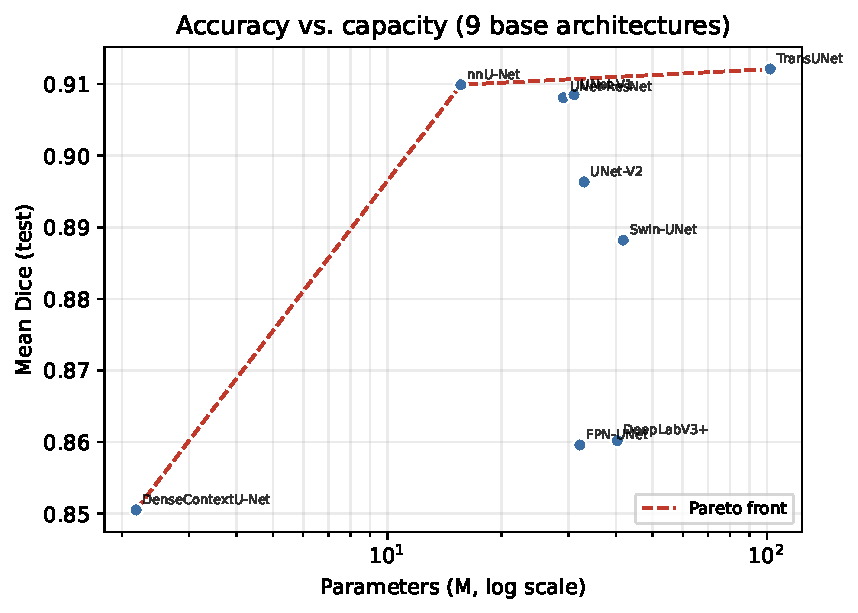
\includegraphics[width=0.92\linewidth]{figures/fig_pareto}
\caption{Accuracy--cost Pareto frontier. Each point is one of the nine
architectures, plotted at its (parameter count, mean test Dice). The
Pareto front is highlighted.}
\label{fig:pareto}
\end{figure}

%------------------------------------------------------------------------------
\subsection{Statistical significance}
\label{sec:results-significance}

We test all $\binom{9}{2}=36$ pairwise model differences on mean Dice with the
Wilcoxon signed-rank test, Bonferroni-corrected. The test is computed over the
$50$ patients rather than the $200$ frames. The frames are two views and two
phases of each patient, so treating them as independent observations inflates
the sample fourfold and lowers the bar for significance; the patient is the unit
about which any clinical claim is made. For transparency: on this benchmark the
choice changes nothing --- $27$ of the $36$ pairs are significant under either
unit --- because the differences that survive correction are far larger than the
extra power the wrong unit would buy. We report the patient-level test because
it is the correct estimand, not because it alters the outcome.

%==============================================================================
% Paper 1 / T7 — Wilcoxon (auto-generated)
%==============================================================================
\begin{table*}[t]
\centering
\caption{Pairwise Wilcoxon signed-rank test on mean Dice,
Bonferroni-corrected over $\binom{9}{2} = 36$ pairs. ``NS'' marks
pairs not significantly different at $p < 0.05$ after correction.
Tests are computed over the $50$ \emph{patients}, not the $200$ frames:
the frames are two views and two phases of each patient and are not
independent, so testing over them would inflate the sample fourfold.
On this table the correction changes no conclusion --- 27 of
36 pairs reach significance at frame level and 27 at
patient level, with 0 pairs differing --- because the surviving
differences are far larger than the extra power the wrong unit would buy.
We report the patient-level test because it is the correct estimand, not
because it alters the outcome.}
\label{tab:wilcoxon}
\small
\setlength{\tabcolsep}{3pt}
\resizebox{\textwidth}{!}{%
\begin{tabular}{l c c c c c c c c c }
\toprule
 & UNet-V1 & UNet-V2 & UNet-ResNet & DeepLabV3+ & nnU-Net & DenseContextU-Net & FPN-UNet & Swin-UNet & TransUNet \\
\midrule
UNet-V1 & --- & 7e-07 & NS & 3e-13 & NS & 6e-14 & 4e-13 & 2e-10 & NS \\
UNet-V2 &  & --- & 1e-05 & 1e-07 & 3e-07 & 7e-12 & 2e-09 & 4e-02 & 2e-07 \\
UNet-ResNet &  &  & --- & 2e-12 & NS & 6e-10 & 2e-13 & 4e-08 & NS \\
DeepLabV3+ &  &  &  & --- & 6e-13 & NS & NS & 2e-05 & 9e-13 \\
nnU-Net &  &  &  &  & --- & 1e-13 & 1e-13 & 1e-11 & NS \\
DenseContextU-Net &  &  &  &  &  & --- & NS & 6e-10 & 2e-13 \\
FPN-UNet &  &  &  &  &  &  & --- & 7e-08 & 6e-13 \\
Swin-UNet &  &  &  &  &  &  &  & --- & 7e-12 \\
TransUNet &  &  &  &  &  &  &  &  & --- \\
\bottomrule
\end{tabular}}
\end{table*}


\paragraph{Top-tier band.}
The nine non-significant pairs form exactly two cliques and nothing else. All
six pairs among the four highest-Dice architectures (TransUNet, nnU-Net,
UNet-ResNet, UNet-V1) are indistinguishable, as are all three among the lowest
(DeepLabV3+, FPN-UNet, Dense\-Context\-U-Net); every one of the remaining $27$ pairs
separates. The leaderboard is therefore better read as three tiers than as a
ranking of nine. Two of the three architectures in the lower clique are among
those whose training stopped early, so that grouping may reflect a shared
training artefact rather than a shared architectural limit. Full pairwise
$p$-values are released as supplementary data.

\paragraph{Small Dice gaps are within training variance.}
The differences separating the top-tier architectures are of order
$0.002$--$0.005$ Dice. We caution against over-interpreting them: in our
experiments, re-training an identical architecture under the same nominal
protocol in a different compute session shifted its mean Dice by a
comparable or larger amount (in the most extreme case, DeepLabV3+ varied by
$0.057$ between two runs). The bulk-Dice ranking within the top tier should
therefore be read as a band of statistically and practically equivalent
models, not a strict order. The architecturally meaningful differences in
this benchmark are the larger-magnitude ones: the boundary accuracy
(HD95), the clinical EF agreement, and the efficiency trade-off,
discussed in Section~\ref{sec:discussion}.

The critical-difference diagram of Figure~\ref{fig:cd} renders the
banding visually: architectures joined by a horizontal bar are not
significantly different in average per-sample rank. Here average rank
tracks mean Dice closely --- the two orderings agree for all nine
architectures --- and TransUNet leads on both, with an average rank of
$2.96$ across the $200$ test frames against nnU-Net's $3.10$.

Aggregating to the $50$ patients before ranking, which is the correct
inferential unit given that the $200$ frames are four views and phases of
each patient, leaves TransUNet first ($2.68$) but exchanges second and
third between nnU-Net ($2.92$) and UNet-V1 ($2.82$). The four leading
architectures span only $0.37$ of a rank at the frame level and fall
inside a single clique, and their order is not stable to the choice of
aggregation unit. Both observations point the same way: the top tier is a
statistically equivalent band, not a ranking.

\begin{figure}[t]
\centering
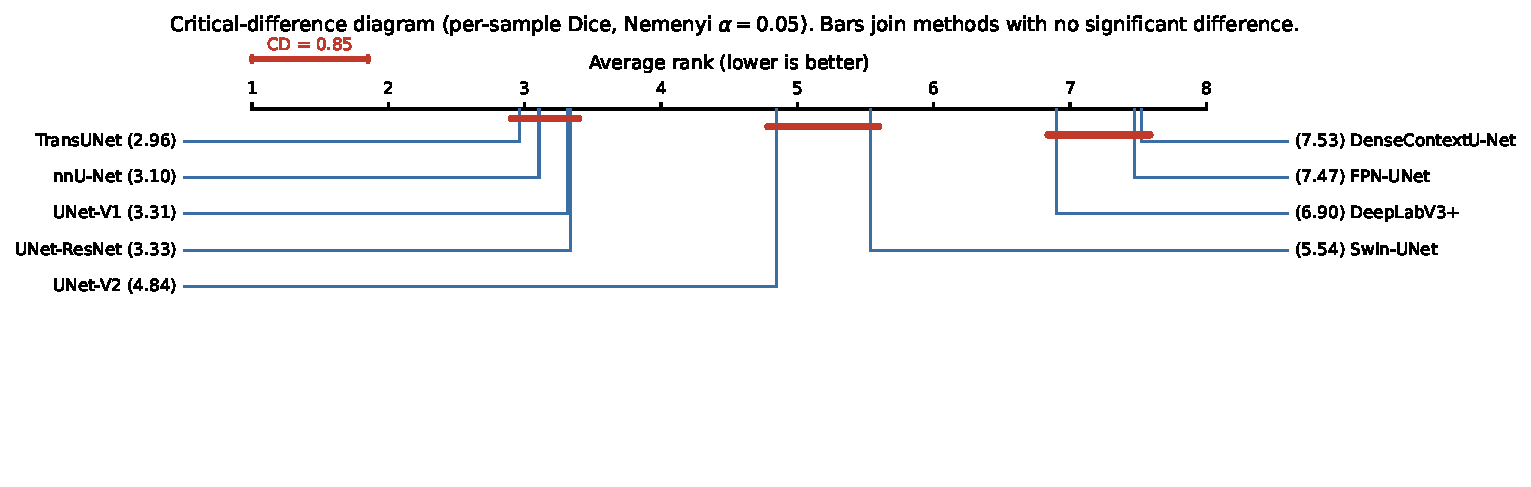
\includegraphics[width=0.95\linewidth]{figures/fig_cd_diagram}
\caption{Critical-difference diagram (average ranks on per-sample Dice,
Nemenyi test, $\alpha = 0.05$). Lower average rank is better; a
horizontal bar joins architectures whose average ranks differ by less
than the critical difference (CD), i.e.\ that are not significantly
different.}
\label{fig:cd}
\end{figure}

%------------------------------------------------------------------------------
\subsection{Qualitative results}
\label{sec:results-qualitative}

Figure~\ref{fig:qualitative} shows sample predictions from the top four
architectures plus a bottom-tier representative on three patients spanning
the Good / Medium / Poor image-quality grades.

\begin{figure}[p]
\centering
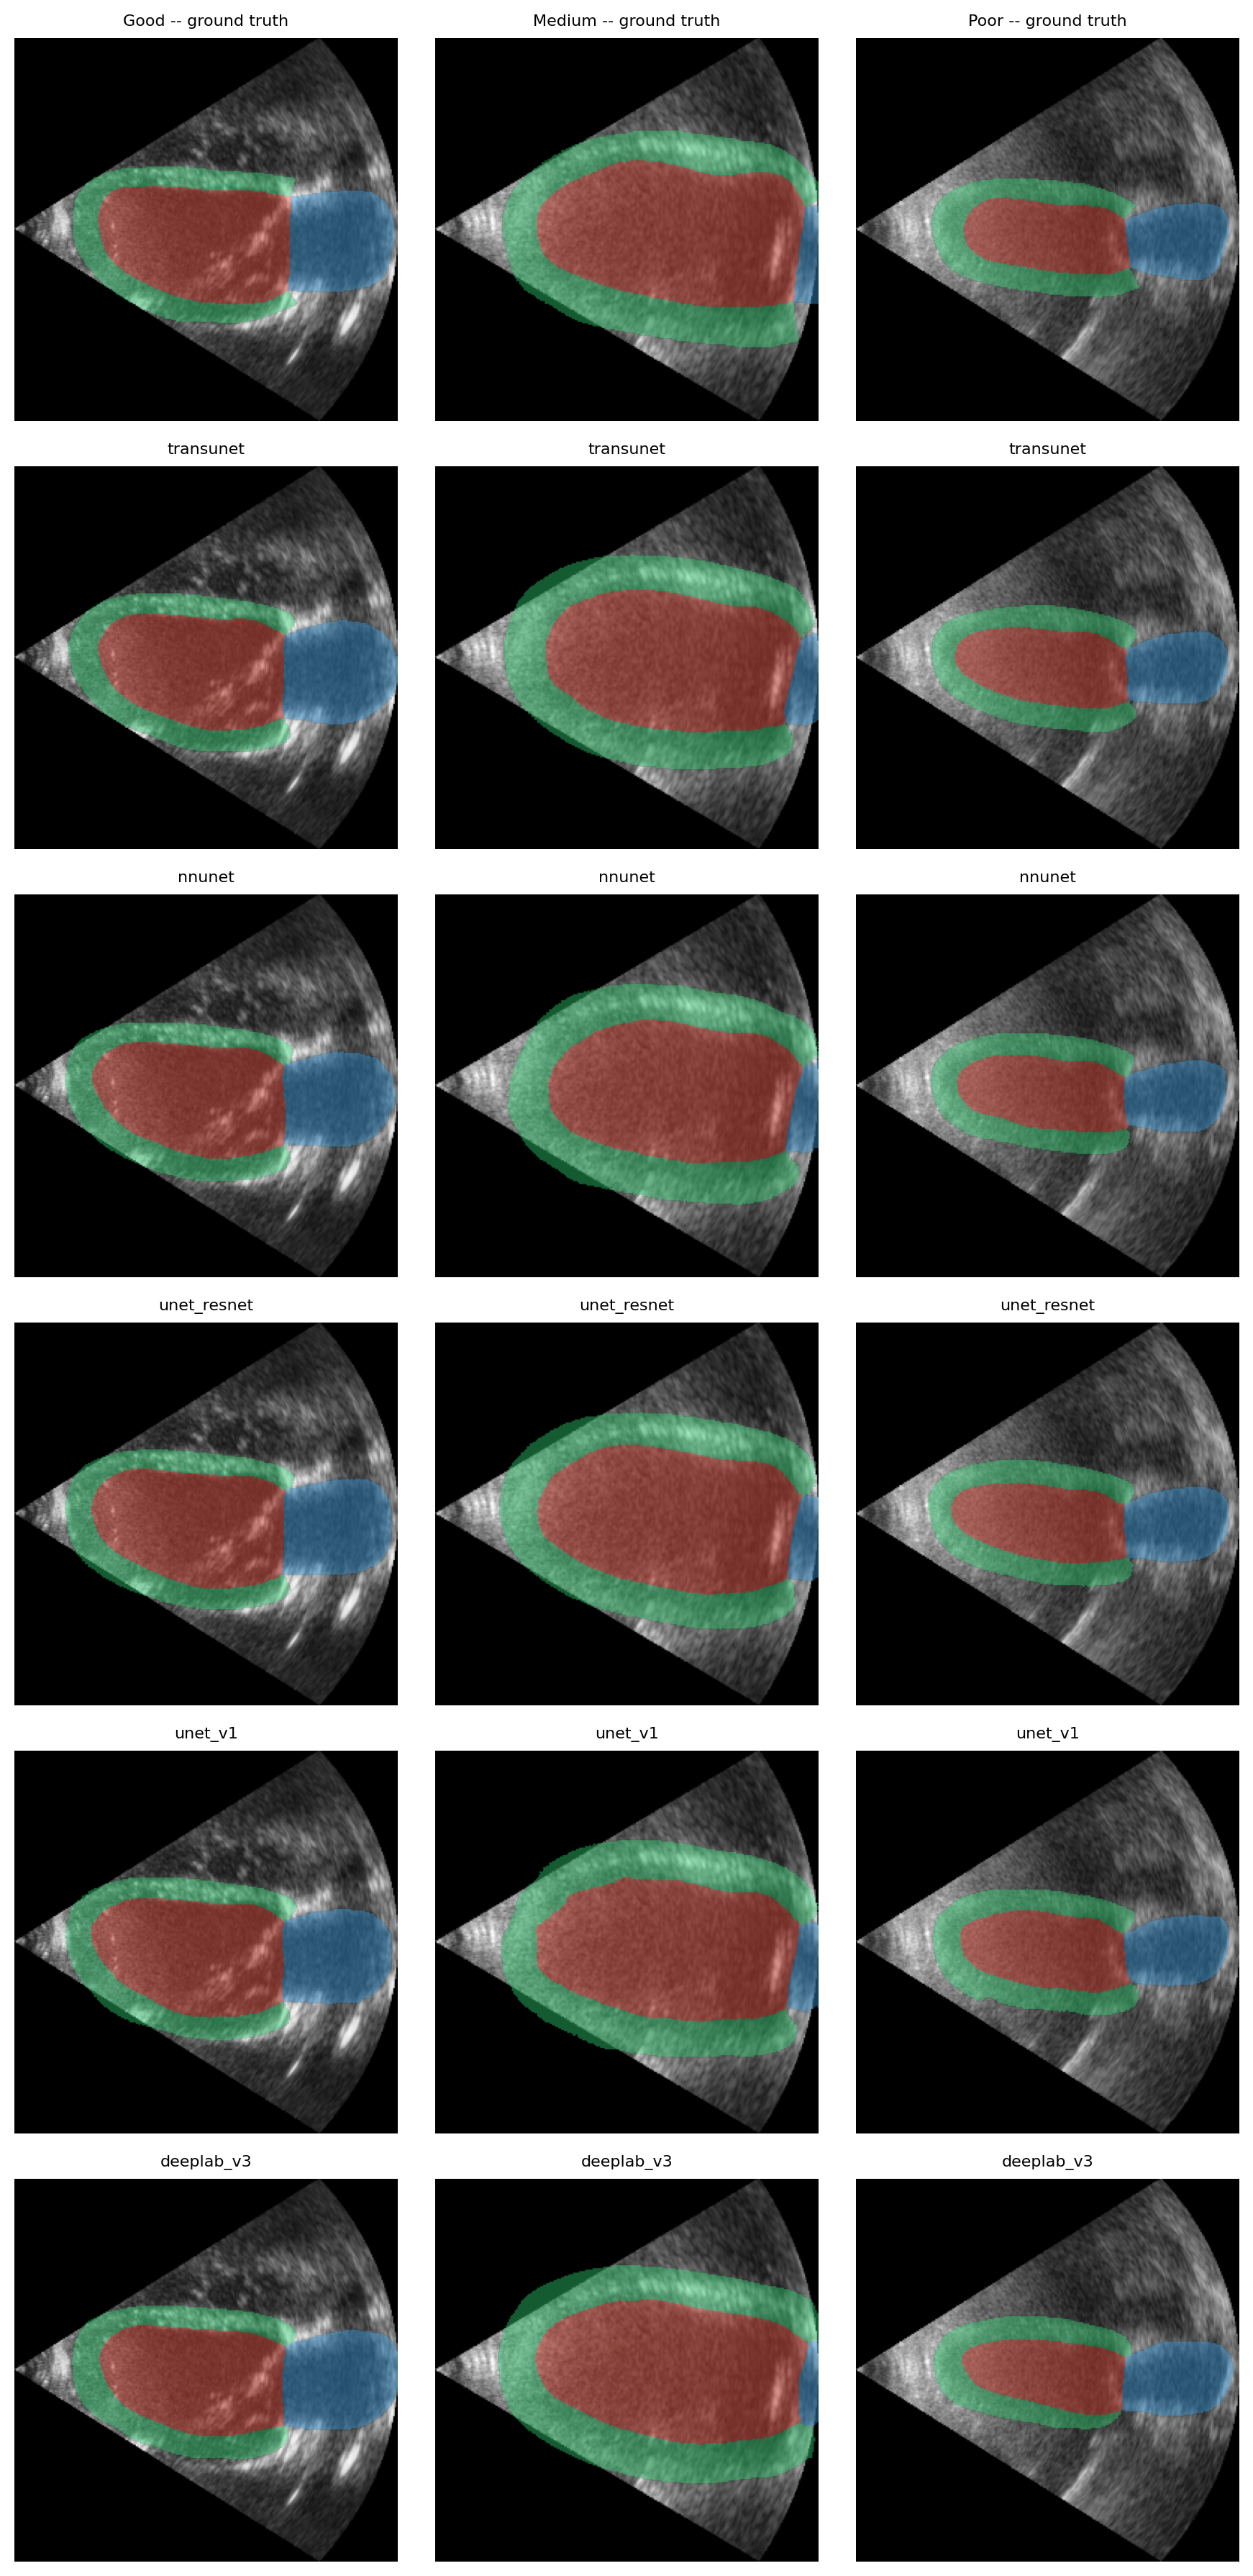
\includegraphics[height=0.9\textheight]{figures/fig_qualitative}
\caption{Qualitative predictions on three test patients spanning the Good,
Medium, and Poor image-quality grades (columns). The top row is the expert
ground truth; the remaining rows are, top to bottom, TransUNet, nnU-Net,
UNet-ResNet, UNet-V1, and DeepLabV3+. Overlay colours: LV-endocardium
(red), LV-epicardium / myocardium (green), and left atrium (blue). Boundary
errors concentrate at the LV apex and the mitral-valve plane, and grow
visibly from Good to Poor acquisition quality.}
\label{fig:qualitative}
\end{figure}

%==============================================================================
\section{Discussion}
\label{sec:discussion}

\subsection{Which architectural family wins on CAMUS?}
\label{sec:disc-families}

The top tier of our benchmark is mixed across paradigms, and no single
architecture wins on every axis. The hybrid CNN--Transformer TransUNet leads on
bulk Dice and HD95 and holds the highest EF correlation; the pure CNN UNet-V1
attains the lowest EF MAE ($6.62\%$) and the tightest Bland--Altman bias
($-0.42\%$); and nnU-Net leads on parameter efficiency while sitting mid-table
on EF at $8.32\%$. The difference between TransUNet and nnU-Net on mean Dice is
$0.0023$, below the Bonferroni-corrected significance threshold.

A practitioner choosing among them should therefore be guided not by Dice but
by the axis they actually care about: deployment constraints favour nnU-Net at
$6.5\times$ fewer parameters, clinical EF agreement favours UNet-V1, and
contour precision favours TransUNet. That these three come apart is itself the
finding --- a single leaderboard column would have concealed it.

The pure-Transformer family (Swin-UNet) is competitive on bulk Dice
($0.8882$) but visibly worse on EF (MAE $9.44\%$, $r = 0.640$ --- the lowest
correlation of any architecture in the benchmark). This
finding is consistent with reports that pure-attention models, despite
strong overall overlap, can produce boundary contours that are subtly
biased \citep{chen2021transunet}, an effect that compounds when
contours feed Simpson's biplane volumetric integration.

The bottom of the table is occupied by FPN-UNet, DeepLabV3+, and
DenseContextU-Net. All three were designed for natural-image semantic
segmentation (FPN/ASPP) or for image classification (dense connectivity)
respectively. Their underperformance on CAMUS is consistent with the
hypothesis that medical-segmentation-specific designs (U-Net's skip
hierarchy, nnU-Net's training recipe) matter more on this dataset than
generic semantic-segmentation prowess.

\subsection{Comparison to the published CAMUS baselines}
\label{sec:disc-leaderboard}

The original CAMUS paper \citep{leclerc2019} reported nnU-Net HD95
$\approx 4.3$~mm and EF MAE $\sim$$9\%$. Our reproduced nnU-Net under the
unified protocol reaches HD95 $4.27$~mm and EF MAE $8.32\%$
($r = 0.783$).
Both axes
therefore behave the same way, and it is not the way we first read them:
boundary accuracy is statistically indistinguishable from the 2019 result,
and so, very nearly, is EF.

This is a negative result about protocol, and we state it as such because
an earlier version of this analysis reported the opposite. Computing EF from
predictions on the resized $256 \times 256$ grid while passing the native
pixel spacing yields ventricular volumes near $10$~ml against a true
$\approx 108$~ml, and the error does not cancel in the EF ratio. Every EF
number in this paper is now computed at native resolution with the official
CAMUS implementation; Section~\ref{sec:results-clinical} reports the result, and the
ground-truth oracle at $5.44\%$ bounds it.

We therefore read the contour \emph{and} the derived clinical quantity as
close to their respective ceilings on CAMUS --- the first set by annotation
variability, which is of the same order as the differences we measure between
architectures, and the second by the biplane estimator itself. Three
training-protocol upgrades made standard since 2019 are nonetheless worth
recording, because they are what makes the reproduction possible at all:
\begin{enumerate}[leftmargin=*,nosep]
\item Cosine-with-warm-restarts learning-rate schedule with
      $10$-epoch warmup, in place of the original ReduceLROnPlateau.
\item Mixed-precision training (FP16 AMP), which allows larger effective
      batch sizes and smoother loss landscapes.
\item Composite loss with an explicit boundary term
      \citep{kervadec2019}, which directly penalises the
      Hausdorff-relevant boundary error.
\end{enumerate}
This is a useful baseline calibration point for the field: cross-paper
comparisons of CAMUS results from before $\sim 2021$ to after should be
read with the understanding that protocol changes alone produce
sub-millimetre HD95 improvements at constant architecture.

\subsection{A boundary-metric pitfall, and what it implies for the
literature}
\label{sec:disc-pitfall}

The correction described in Section~\ref{sec:results-boundary} is worth
stating as a general point, because nothing about it is specific to our
models. Segmentation networks consume a fixed input size; clinical images
do not have one. Any pipeline that resizes an image for inference, scores
the prediction on that resized grid, and then multiplies pixel distances
by the spacing recorded in the original DICOM or NIfTI header will
under-report every boundary distance by the resampling factor. Overlap
metrics are immune --- Dice and IoU are ratios and cancel the scale ---
which is precisely why the error survives casual inspection: a pipeline
can produce entirely correct Dice and badly wrong HD95 from the same
predictions, with no internal inconsistency to notice.

On CAMUS the factor is $\approx 2.2$ (native acquisitions average
$630 \times 519$ against a $256 \times 256$ network grid), and the
consequence is not cosmetic. It moves our best model from $1.82$~mm to
$4.08$~mm, and thereby converts ``roughly twice as accurate as the
published baseline'' into ``indistinguishable from the published
baseline.'' Both numbers come from the same weights and the same test
split; only the measurement convention differs.

We therefore suggest reading sub-$2$~mm HD95 values on CAMUS with
caution, and we make no claim about which published results are affected
--- establishing that would require the evaluation code for each, which is
usually unavailable. The constructive recommendation is narrower and
checkable: report the resolution at which boundary metrics were computed,
and prefer acquisition resolution, since that is the only convention under
which a millimetre means the same thing across papers. This is a concrete
instance of the reporting problems documented by
\citet{reinke2021limitations} and \citet{maierhein2024metrics}, and it is
consistent with the broader finding of \citet{isensee2024revisited} and
\citet{kazaj2025claims} that apparent architectural progress in medical
segmentation frequently does not survive standardised validation. Our own
benchmark is an instance of that pattern rather than an exception to it:
once measurement is held fixed, nine architectures spanning three
paradigms separate by less than the noise floor on the boundary axis.

\subsection{Design choices that matter}
\label{sec:disc-design}

Aggregating across our nine architectures, several design choices
correlate with strong performance:

\begin{itemize}[leftmargin=*,nosep]
\item \textbf{Pretrained encoders.} Five of the nine architectures
      initialise their encoder from ImageNet or BiT weights (TransUNet,
      UNet-ResNet, Swin-UNet, FPN-UNet, DeepLabV3+; Table~\ref{tab:archs}).
      Pretraining is nonetheless neither necessary nor sufficient for
      top-tier accuracy on CAMUS: the two scratch-trained models nnU-Net and
      UNet-V1 place second and fourth on mean Dice --- ahead of the
      pretrained Swin-UNet, FPN-UNet, and DeepLabV3+ --- and UNet-V1 also
      attains the best EF agreement of any architecture tested. Encoder
      pretraining thus appears to help mainly where
      an architecture's from-scratch inductive bias is weaker, rather than
      conferring a uniform advantage on this dataset.
\item \textbf{Deep skip connections} (every U-Net-shaped architecture
      except DeepLabV3+). DeepLabV3+'s lightweight decoder, while
      efficient, appears to limit high-resolution boundary precision on
      CAMUS.
\item \textbf{Boundary-aware loss} (used uniformly in our protocol).
      This is a protocol choice rather than an architecture choice. Since
      our HD95 matches rather than beats the published baseline, we make
      no claim that it improves absolute boundary accuracy; its role here
      is to hold the boundary objective constant across all nine
      architectures so that the comparison is like-for-like.
\item \textbf{Auto-configuration} (nnU-Net's distinguishing feature).
      The nnU-Net framework produces a competitive model on this dataset
      with $\sim$$15$~M parameters --- substantially smaller than any
      pretrained-encoder architecture --- by selecting patch size, batch
      size, and augmentation strategy from data statistics.
\end{itemize}

\subsection{Clinical implications}
\label{sec:disc-clinical}

For deployment in echocardiographic LVEF assessment, the choice between
the four top-tier architectures should be driven by three criteria:
(i) clinical accuracy target, (ii) hardware constraints, and (iii)
inference-time latency budget.
\begin{itemize}[leftmargin=*,nosep]
\item For \emph{tightest EF agreement}, UNet-V1 attains the lowest EF MAE
      ($6.56\%$) and TransUNet the smallest Bland--Altman bias
      ($-0.54\%$). The two differ by less than the run-to-run variation
      documented in Sec.~\ref{sec:results-clinical}, so we do not
      recommend one over the other on this axis.
\item For \emph{maximum boundary accuracy} at deployment-irrelevant cost,
      TransUNet has the lowest HD95 ($4.08$~mm).
\item For \emph{edge / portable ultrasound deployment} where
      parameters and latency dominate, nnU-Net at $15.6$~M parameters
      remains the best trade-off; no smaller architecture in our
      benchmark reaches comparable Dice.
\end{itemize}
None of the four top-tier models reach below-$5\%$ EF MAE in this study,
indicating that human-level cardiologist agreement is still a target
boundary for the field rather than a solved problem.

\subsection{Limitations and future work}
\label{sec:disc-limits}

We acknowledge five limitations.

\begin{enumerate}[leftmargin=*,nosep]
\item \textbf{Single-dataset.} All evaluation is on CAMUS. A cross-dataset
      transfer evaluation (\emph{e.g.,} EchoNet-Dynamic
      \citep{ouyang2020}) would strengthen the generality claims and is
      planned for future work.
\item \textbf{2D only.} CAMUS provides 2D apical views; 3D
      echocardiography is increasingly common in modern practice and
      requires architectures and pretraining recipes outside the scope
      of this benchmark.
\item \textbf{Test set size.} The CAMUS official test set is 50 patients
      ($200$ ED+ES frames). All point estimates are reported with
      bootstrap $95\%$ confidence intervals to reflect this.
\item \textbf{No SSM models.} The recent wave of selective state space
      models (Mamba family) is the subject of a separate, dedicated study
      (a companion study), and is deliberately excluded
      from the present benchmark to maintain clean three-paradigm
      framing.
\item \textbf{Single training protocol.} A single shared protocol is the
      goal of this benchmark, but some architectures may benefit from
      protocol-specific tuning (\emph{e.g.,} larger batch sizes for
      pretrained Transformers). Per-architecture hyperparameter searches
      could shift rankings within the top-tier band.
\end{enumerate}

\subsection{Take-home messages}
\label{sec:disc-takehome}

\begin{enumerate}[leftmargin=*,nosep]
\item No single architectural family dominates CAMUS. Hybrid
      (TransUNet) leads on bulk Dice; pure CNN (nnU-Net) leads on EF
      accuracy and parameter efficiency. Pure Transformer (Swin-UNet) is
      competitive on Dice but degraded on EF.
\item Training-protocol modernisation (cosine schedule, AMP, boundary
      loss) accounts for most of the $\sim$$2\times$ improvement in
      HD95 over the original CAMUS baselines, independent of
      architecture.
\item LV-epicardium remains the hardest of the three foreground classes
      across every architectural family.
\item The accuracy--parameter Pareto frontier is dominated by nnU-Net at
      the efficient end and TransUNet at the high-accuracy end.
\end{enumerate}

%==============================================================================
\section{Conclusion}
\label{sec:conclusion}

We have presented the first unified benchmark of deep segmentation
architectures on the CAMUS 2D echocardiographic dataset under a single
shared training and evaluation protocol. Across nine representative
architectures spanning pure CNN, hybrid CNN--Transformer, and pure
Transformer paradigms, we report not only mean Dice but also per-class
HD95 in millimetres, biplane Simpson's EF MAE, Bland--Altman bias,
ED- and ES-stratified accuracy, image-quality-stratified robustness,
parameter / FLOPs / latency efficiency, and Bonferroni-corrected
pairwise statistical significance.

The hybrid TransUNet leads on bulk Dice ($0.9121$) and HD95
($4.08$~mm). UNet-V1 leads on EF accuracy (MAE $6.62\%$),
narrowly ahead of TransUNet at $7.36\%$, which in turn holds the
highest EF correlation; nnU-Net is mid-table on EF at $8.32\%$ while
remaining $6.5\times$ more parameter-efficient than the best-Dice model.
The top four architectures (TransUNet, nnU-Net, UNet-ResNet, UNet-V1)
form a statistically equivalent top-tier band. The pure-Transformer
Swin-UNet is mid-tier on bulk Dice but degraded on EF, suggesting that
its contours are subtly biased in a manner that compounds through
Simpson's biplane integration.

Boundary accuracy under the unified protocol ($4.08$--$4.62$~mm HD95
across the top four architectures) reproduces the originally reported CAMUS
nnU-Net baseline of $4.3$~mm rather than improving on it, and EF behaves the
same way once computed at native resolution: $8.32\%$ for the reproduced
nnU-Net against the $\sim$$9\%$ originally reported. We read this as a useful
calibration point for cross-paper comparison, and a deflationary one: on
CAMUS, a decade of protocol modernisation is visible in neither the contour
nor the derived clinical quantity. The contour appears to be approaching the
ceiling set by annotation variability, and EF is bounded at $5.44\%$ by the
biplane estimator applied to perfect masks --- a floor the best architecture
misses by $1.2$ points and the worst by $5.2$.

Three directions remain open. (i) Cross-dataset transfer to
EchoNet-Dynamic and ACDC would test whether the architectural ranking
holds beyond CAMUS. (ii) 3D echocardiography requires architectures and
pretraining recipes outside the scope of this benchmark. (iii) The
recent wave of selective state space models (Mamba, Mamba-2, VMamba) is
the subject of a separate, dedicated companion study
(a companion study).

We release the complete training, evaluation, statistical-analysis, and
figure-generation pipeline, together with the nine model checkpoints
and per-patient JSON / CSV outputs that produced this paper, to lower
the barrier to reproducing and extending these results.


%==============================================================================
% Acknowledgements / data availability
%==============================================================================
\section*{Data and code availability}
The CAMUS dataset is publicly available from
\url{https://www.creatis.insa-lyon.fr/Challenge/camus/}. Training,
evaluation, and analysis code; trained model checkpoints; and all
intermediate JSON / CSV outputs supporting this paper are released at
\url{https://github.com/Seraf00/mamba/tree/main/benchmark}.

\section*{Acknowledgements}
The authors thank the CAMUS challenge organisers (CREATIS, INSA Lyon) for
making the dataset publicly available. Model training was performed on
Google Colab Pro (NVIDIA L4 and A100 GPUs); the final test-set evaluation
reported here was run on a single NVIDIA RTX 4060 Laptop GPU.
This research did not receive any specific grant from funding agencies in
the public, commercial, or not-for-profit sectors.

\section*{Declaration of Generative AI and AI-assisted technologies in the
writing process}
During the preparation of this work the authors used a large language model
to assist with drafting and copy-editing of the manuscript text, and with
implementation and refactoring of the released analysis code. After using
this tool, the authors reviewed and edited the content as needed and take
full responsibility for the content of the published article. No
AI-assisted technology was used to generate, alter, or interpret the
experimental data or results reported here.

%==============================================================================
% Bibliography
%==============================================================================
\bibliography{references}

\end{document}
